% !TEX encoding = UTF-8
% !TEX TS-program = pdflatex
% !TEX root = ../tesi.tex

%**************************************************************
\chapter{Tecnologie utilizzate}
\label{tecnologie}
%**************************************************************

\section{TypeScript}

\begin{figure}[H] 
  \centering 
  
\includegraphics[width=0.25\columnwidth]{ts} 
  \caption{TypeScript}
\end{figure}

TypeScript è un linguaggio di programmazione open-source sviluppato e mantenuto da Microsoft. La sua sintassi è un super-set di JavaScript, ovvero qualsiasi sintassi di quest'ultima è valida anche nella prima ma non vice-versa. TypeScript aggiunge difatti la possibilità di avere tipi statici. \\

È inoltre progettato per lo sviluppo di grandi applicazioni e compila in JavaScript, per cui può essere usato sia per l'esecuzione lato client che server (Node.js). \\

Il linguaggio fornisce i tipi statici attraverso \textit{type annotations} che attivano il controllo dei tipi a tempo di compilazione. La scelta è tuttavia opzionale ed è possibile scrivere normale codice JavaScript senza tipi. \\

\begin{lstlisting}[language={[Sharp]C}]
// Esempio di funzione con tipi statici
function add(left: number, right: number): number {
  return left + right;
}
\end{lstlisting}

I tipi statici possono anche essere esportati dopo la compilazione in file di dichiarazione separati, in modo da fornire le informazioni sui tipi a chi deve utilizzare la libreria, la quale sarà già stata compilata in JavaScript. \\

Sia la libreria \textit{Stargate} che l'applicazione \textit{WorkWave Route Manager} sono scritte in TypeScript 3.0, rilasciato ad agosto 2018.

\section{React}

\begin{figure}[H] 
  \centering 
  
\includegraphics[width=0.25\columnwidth]{react} 
  \caption{React}
\end{figure}

\textbf{React} è una libreria JavaScript per la realizzazione di applicazioni web, in particolare per la creazione di interfacce utenti. È mantenuta e sviluppata da Facebook, sebbene abbia anche una forte community open-source. \\

La seguente classe è un componente UI React, che accetta una proprietà \texttt{greeting}. Il metodo \texttt{ReactDOM.render} si occupa invece di creare un'istanza di tale componente, passando ad esso \texttt{"Hello World!"} come valore di \texttt{greeting}. Il risultato è renderizzato come figlio del nodo HTML avente id \texttt{"root"}. \\

\begin{lstlisting}[language={[Sharp]C}]
class Greeter extends React.Component { 
  render() { 
    return <h1>{this.props.greeting}</h1>
  } 
} 

ReactDOM.render(
  <Greeter greeting="Hello World!" />,
  document.getElementById('root')
);
\end{lstlisting}

Di seguito sono invece elencate le caratteristiche principali di React, che hanno fortemente influenzato lo sviluppo moderno di web applications:

\begin{itemize}
  \item \textbf{One-way data binding con "props"}: tutte le informazioni esterne di cui ha bisogno il componente sono ricevute ed aggiornate tramite \texttt{props} dal componente genitore. Ciò assicura un flusso dei dati unidirezionale e predicibile. Inoltre le \texttt{props} sono da trattarsi come dati in sola lettura ed immutabili;
  \item \textbf{Componenti Stateful}: oltre alle \texttt{props}, i componenti possono avere uno stato interno utilizzabile internamente o passabile come \texttt{prop} ai figli.

  \vfill

    \begin{lstlisting}[language={[Sharp]C}]
class ParentComponent extends React.Component {
  state = { color: 'red' };

  render() {
    return (
      <ChildComponent color={this.state.color} />
    );
  }
}
    \end{lstlisting}

  \item \textbf{Virtual DOM}: il DOM è la rappresentazione in JavaScript della struttura HTML della pagina. React crea invece una propria rappresentazione virtuale del DOM dei propri componenti ed aggiorna efficientemente quello reale solo laddove necessario. Ciò consente al programmatore di descrivere il \texttt{render} dell'intera applicazione in base a \texttt{props} e \texttt{state}, mentre React si occupa delle effettive modifiche necessarie al DOM;
  \item \textbf{JSX}: è un'estensione della sintassi JavaScript per poter scrivere un codice simile all'HTML, ma dinamicamente in JavaScript, invece che come stringa template statica.
\end{itemize}

React può essere usato come libreria di appoggio per lo sviluppo di applicazioni sia web che mobile e spesso è accompagnata da ulteriori librerie, quali \textit{Redux}, per la gestione dello stato, delle rotte o delle richieste server.

\section{Redux}

\begin{figure}[H] 
  \centering 
  
\includegraphics[width=0.25\columnwidth]{redux} 
  \caption{Redux}
\end{figure}

\textbf{Redux} è una libreria JavaScript per la gestione dello stato applicativo, che può essere visto come l'equivalente dello stato di un componente React ma relativo all'intera applicazione. La libreria implementa l'architettura \textit{Flux}, un'alternativa al popolare Model-View-Controller e che si avvicina più ad architetture ad eventi/messaggi. \\

In Redux, oggetti chiamati \textit{actions} hanno il compito di descrivere l'intento di modifica dello stato applicativo. Tale messaggio viene inviato allo \textit{Store}, il quale gestisce la modifica dello stato applicativo in base all'\textit{action} e notifica la view (React) del cambiamento. Nessuna classe, ad eccezione dello \textit{Store}, ha la possibilità quindi di aggiornare lo stato applicativo, trattato come immutabile. \\

All'interno dello \textit{Store}, l'aggiornamento effettivo dello stato applicativo avviene attraverso i \textit{reducers}, funzioni pure aventi la firma \texttt{(State, Action) => State} e componibili tra di loro. \\

Si genera quindi un flusso unidirezionale, in cui la view riceve i dati e notifica di eventi tramite \textit{actions}. Quest'ultimi sono passati ai \textit{reducers} che producono un nuovo stato applicativo, passato dallo \textit{Store} nuovamente alla view.

\begin{figure}[H] 
  \centering 
  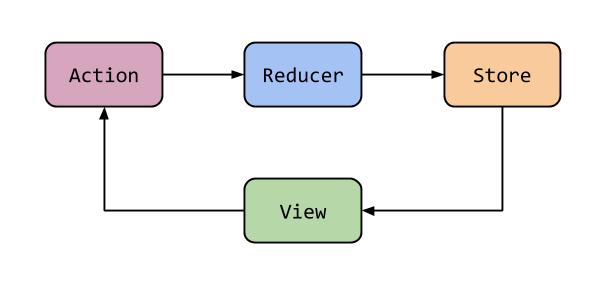
\includegraphics[width=0.75\columnwidth]{flux} 
  \caption{Flusso unidirezionale in Redux}
\end{figure}
